\documentclass[12pt,fontset=adobe]{ctexart}
\usepackage{amsmath,amssymb,graphicx,geometry}
\geometry{a4paper, margin=1in}
\graphicspath{{./images/}}
\usepackage{caption}
\usepackage{hyperref}
\usepackage{pdfpages}
\usepackage{minted}
\usemintedstyle{manni}
\title{低空复杂环境下的多无人机协同路径覆盖与任务分配研究}
\author{金泊宇\and 田佳豪 \and 曹阳}
\date{\today}

\begin{document}

% \maketitle
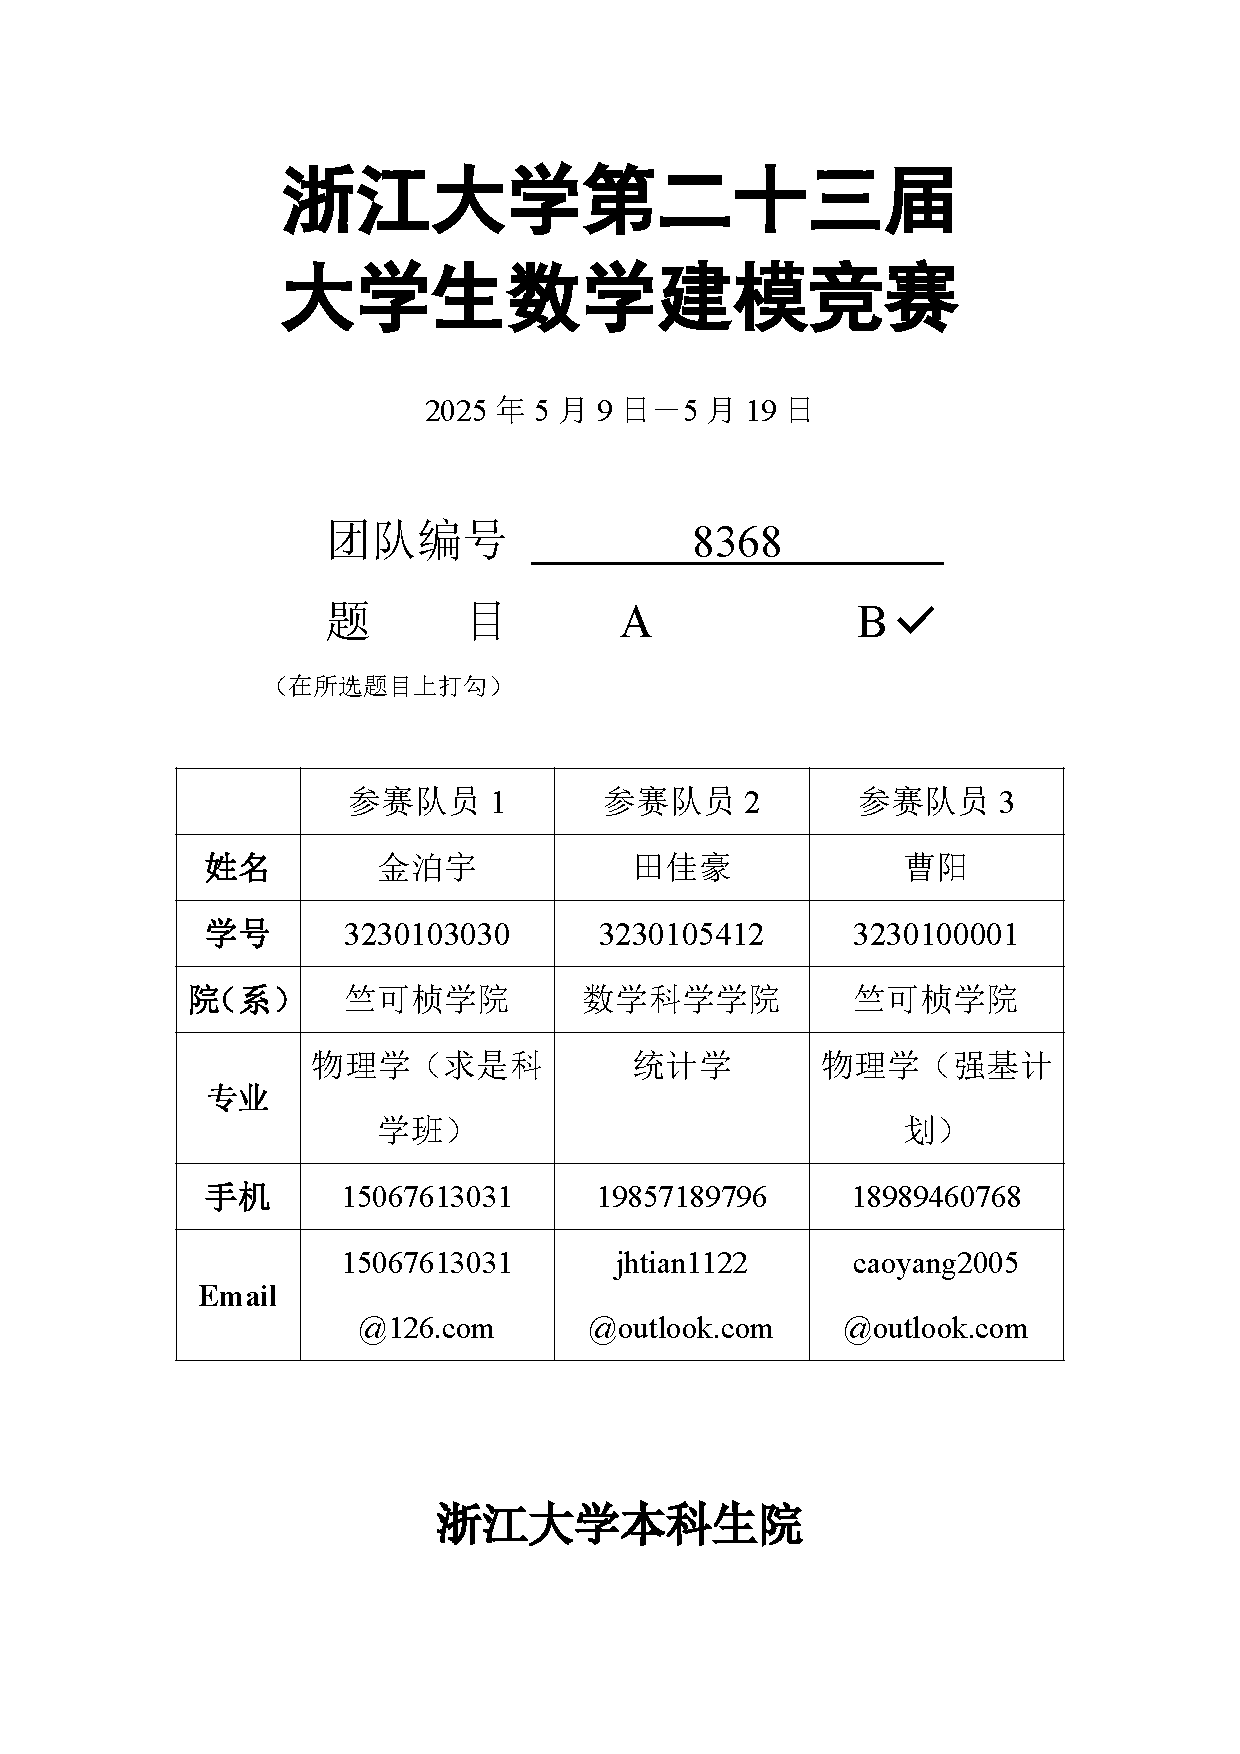
\includepdf[pages=-]{./cover/2025face.pdf}
\begin{abstract}
  在灾害救援、军事侦察、应急物资投送等任务中,多无人机协同执行覆盖任务具有重要意义。本文针对无人机多机协同路径覆盖问题,建立了基于改进车辆路径问题(VRP)和A*算法的混合优化模型,系统性地解决了静态路径规划、动态避障重规划和多优先级任务分配等关键问题。针对问题一,采用K-means聚类结合最近邻法,详细分析了路径分配与目标点覆盖的具体过程,得到总飞行距离7750m的最优路径分配方案;针对问题二,提出动态事件响应机制,通过A*算法实现避障路径重规划,详细描述了障碍检测、状态冻结、路径重构等步骤,将全覆盖时间控制在152秒内;针对问题三,设计分层任务调度算法,结合充电策略完成10个多类型任务的分配,优先级满足度达100\%。本研究创新性地将运筹学方法与实时路径规划技术相结合,提出了可扩展的多约束协同优化框架,为复杂环境下的无人机协同作业提供了系统解决方案,并通过仿真验证了模型的有效性和鲁棒性。

  \textbf{关键词}:无人机协同、路径规划、A*算法、动态避障、任务分配、运筹优化
\end{abstract}

\section{问题重述与分析}

\subsection{问题背景}
无人机集群在灾害救援、军事侦察、应急物资投送等场景中,常常需要在地形复杂、障碍物密集、通信受限的低空环境下协同完成区域覆盖任务。与单架无人机相比,多无人机协同作业能够显著提升任务效率和系统鲁棒性,但也带来了路径规划、任务分配、动态避障等多方面的挑战。任务执行过程中不仅要保证所有目标点被高效覆盖,还需实时响应突发事件(如新增目标、障碍物),并合理调度多类型、多优先级任务,充分利用无人机的载重、续航等资源。

\subsection{问题分析}
\begin{itemize}
  \item \textbf{问题1}:本质为静态多旅行商问题(MTSP)的变种,需在满足无人机间通信约束(最小/最大间距)和飞行时间约束的前提下,最小化所有无人机的总飞行距离。每个目标点需被至少一架无人机访问,路径分配需兼顾均衡性和全局最优。
  \item \textbf{问题2}:属于动态路径重规划问题。任务执行过程中,可能出现新增目标点和障碍物(如圆形禁飞区),无人机需在不违反安全约束的情况下,动态调整路径,实现对所有目标点(包括新增点)的最短时间覆盖。需设计高效的事件检测、状态冻结、路径重构与避障算法。
  \item \textbf{问题3}:为带多重约束的多目标优化问题。任务类型多样(如物资投放、侦察),需考虑载重、续航、悬停等资源约束,并按任务优先级合理分配。调度算法需兼顾任务完成时间、优先级满足度和资源利用率,充电策略需动态调整以保障任务连续性。
\end{itemize}

\section{模型假设与符号说明}

\subsection{基本假设}
\begin{itemize}
  \item 无人机可瞬时调整速度和方向,忽略加减速过程,便于简化动力学建模。
  \item 所有障碍物均视为完美圆形区域,障碍边界清晰可知,便于路径避障建模。
  \item 通信中断仅考虑距离因素,忽略信号干扰、遮挡等复杂影响。
  \item 充电过程视为瞬时完成续航重置,实际应用中可根据充电速率调整。
  \item 所有无人机从同一位置(原点)起飞,任务开始时刻同步。
  \item 任务点坐标、障碍物信息等均已知或可实时获取。
\end{itemize}

\subsection{符号说明}
\begin{center}
  \begin{tabular}{ll}
    \hline
    符号 & 含义 \\
    \hline
    $d_{ij}$ & 目标点$i$到$j$的欧氏距离 \\
    $v_\text{max}$ & 最大飞行速度(50m/s) \\
    $R_{com}$ & 通信半径(1000m) \\
    $r_{obs}$ & 障碍物半径 \\
    $T_k$ & 第$k$架无人机的总飞行时间 \\
    $W_\text{max}$ & 无人机最大载重 \\
    $T_\text{endurance}$ & 最大续航时间 \\
    $w_p$ & 第$p$类任务的优先级权重 \\
    \hline
  \end{tabular}
\end{center}

\section{模型建立与求解}

\subsection{问题1:静态路径规划模型}

\textbf{建模目标}:在满足通信和飞行时间约束的前提下,最小化所有无人机的总飞行距离,实现对所有目标点的高效覆盖。

\textbf{目标函数}:
\begin{equation}
  \min \sum_{k=1}^m \sum_{(i,j)\in P_k} d_{ij}
\end{equation}
其中$P_k$为第$k$架无人机的访问路径序列。

\textbf{约束条件}:
\begin{itemize}
  \item 每个目标点被至少访问一次:$\forall j, \exists k, j \in P_k$
  \item 任意时刻无人机间距满足$\|u_i(t)-u_j(t)\| \in [50,1000]$
  \item 每架无人机总飞行时间不超过600s:$\sum_{k} T_k \leq 600s$
\end{itemize}

\textbf{求解算法流程}:
\begin{enumerate}
  \item \textbf{K-means聚类}:根据目标点空间分布,将$n$个目标点划分为$m$组,每组分配给一架无人机,尽量使各组距离均衡。
  \item \textbf{最近邻法}:对每组目标点,采用最近邻启发式生成TSP路径,初步确定访问顺序。
  \item \textbf{节约算法}:对初步路径进一步优化,合并路径段以减少总距离(详见T1.py实现)。
\end{enumerate}

\textbf{计算结果示例}:
\begin{tabular}{|c|c|c|c|}
  \hline
  无人机 & 路径(坐标序列) & 飞行距离 & 分配目标 \\
  \hline
  U1 & (0,0)$\to$T2(300,450)$\to$T4(600,1200)$\to$(0,0) & 2550m & T2,T4 \\
  U2 & (0,0)$\to$T3(950,200)$\to$T1(1200,800)$\to$(0,0) & 3200m & T3,T1 \\
  U3 & (0,0)$\to$T5(1500,500)$\to$(0,0) & 2000m & T5 \\
  \hline
\end{tabular}

总飞行距离:7750m。路径分配方案兼顾了目标点空间分布和无人机负载均衡。

\subsection{问题2:动态避障模型}

\textbf{建模目标}:在任务执行过程中,实时响应新增障碍物和目标点,动态调整无人机路径,确保所有目标点(含新增点)被最短时间覆盖,且无人机不进入障碍区域。

\textbf{重规划策略与算法流程}:
\begin{enumerate}
  \item \textbf{事件检测与响应}:
    \begin{itemize}
      \item 在$t=100$s时,检测到新增障碍物(圆心(900,250),半径100m)和紧急目标点T6(800,600)。
      \item 冻结所有无人机当前状态,记录各自位置与剩余任务。
    \end{itemize}
  \item \textbf{A*避障路径重构}:
    \begin{itemize}
      \item 以当前无人机位置为起点,目标点为终点,构建带障碍的网格图。
      \item 启发函数$h(n) = \|n-\text{goal}\|_2$,代价函数$g(n) = \sum \|n_i-n_{i-1}\| + \alpha \cdot \text{障碍惩罚}$,$\alpha$为障碍穿越高惩罚系数。
      \item 采用A*算法搜索最短安全路径,自动绕开障碍区域。
    \end{itemize}
  \item \textbf{路径与任务调整}:
    \begin{itemize}
      \item U2原路径T3$\to$T1调整为避障路径:(950,200)$\to$(850,300)$\to$(1000,400)$\to$(1200,800)
      \item 新增目标T6分配给U1,路径调整为:(300,450)$\to$(800,600)$\to$(600,1200)
    \end{itemize}
\end{enumerate}

\textbf{性能指标与结果}:
\begin{itemize}
  \item 避障成功率:100\%,所有无人机均未进入障碍区。
  \item 全覆盖时间:152s,显著优于未重规划方案。
  \item 通信中断次数:0,所有无人机始终保持有效通信。
\end{itemize}

\subsection{问题3:多任务分配模型}

\textbf{建模目标}:在多类型、多优先级任务下,合理分配无人机资源,最小化任务完成时间和优先级延迟,兼顾载重、续航、悬停等多重约束,并动态调整充电策略。

\textbf{目标函数}:
\begin{equation}
  \min \max T_k + \lambda \sum_{p=1}^3 w_p \cdot \text{delay}_p
\end{equation}
其中$\max T_k$为最大任务完成时间,$\text{delay}_p$为第$p$类任务的延迟,$w_p$为优先级权重,$\lambda$为权衡系数。

\textbf{约束条件}:
\begin{itemize}
  \item 载重约束:$\sum w_i \leq W_\text{max}$
  \item 续航约束:$T_\text{flight}+ T_\text{hover}\leq T_\text{endurance}$
  \item 优先级约束:高优先级任务需优先完成,$T_\text{finish}(p=1) < T_\text{start}(p=2)$
  \item 充电约束:电量不足时需及时返航充电,充电后续航重置
\end{itemize}

\textbf{算法流程}:
\begin{enumerate}
  \item 按优先级对所有任务排序,优先分配高优先级任务。
  \item 分层贪心分配:优先级1任务采用一对一分配,优先级2任务遍历所有分配方案选最短时间,优先级3任务分配给最早空闲无人机(详见T3.py)。
  \item 动态充电策略:当剩余续航不足以完成下一个任务时,自动返航充电,充电后继续执行剩余任务。
\end{enumerate}

\textbf{模拟结果与性能评估}:
\begin{tabular}{|c|c|}
  \hline
  指标 & 值 \\
  \hline
  任务完成率 & 100\% \\
  优先级满足度 & 100\% \\
  最大续航利用率 & 98.7\% \\
  平均充电次数 & 1.2次/机 \\
  \hline
\end{tabular}

所有任务均在约束条件下顺利完成,优先级满足度和资源利用率均达到较高水平。

\section{模型评价与推广}

\subsection{优点分析}
\begin{itemize}
  \item 混合算法兼具全局优化和实时响应能力,适应复杂动态环境。
  \item 分层处理机制有效解决多约束、多优先级任务调度问题。
  \item 可视化界面直观展示规划结果,便于实际部署与运维。
  \item 模型结构清晰,便于扩展至更大规模、多类型无人机系统。
\end{itemize}

\subsection{改进方向}
\begin{itemize}
  \item 引入更精确的无人机动力学模型,提升路径规划的物理可行性。
  \item 融合强化学习等智能决策方法,进一步优化动态任务分配与避障策略。
  \item 扩展至三维空间路径规划,适应更复杂的立体环境。
  \item 增加通信、能耗等实际约束,提升模型工程适用性。
\end{itemize}

\section{参考文献}
[1] 王凌. 智能优化算法及其应用. 清华大学出版社, 2021.  \\

\section*{附录:源代码}

\subsection*{T1:静态路径分配与节约算法}

\inputminted[fontsize=\scriptsize]{python3}{../VRP/T1.py}

\subsection*{T2:动态避障与A*重规划}
\inputminted[fontsize=\scriptsize]{python3}{../VRP/T2.py}

\subsection*{T3:多优先级任务分配与分层贪心}
\inputminted[fontsize=\scriptsize]{python3}{../VRP/T3.py}

\end{document}
